\section{SISTEMA WEB}

A seguir destaca-se as principais telas do sistema web proposto por este
projeto, descrevendo e comparando as características da ferramenta com a antiga
abordagem de gerenciamento das questões que anteriormente ocorria através do
\textit{Google Groups}.

Na Figura \ref{fig:zcpeHome}, exibe-se a página inicial do sistema que apresenta
três maneiras de uso da plataforma, são elas:

\begin{alineas}
    \item anonimamente: permite que o usuário acesse a aplicação sem que haja
    autenticação, liberando acesso para que o usuário gere um template de e-mail
    para disparar manualmente através de seu cliente de e-mail pessoal;
    \item com usuário e senha: permite que o usuário acesse a aplicação com as
    suas credenciais, isto dá direitos para que o usuário gerencie as suas
    próprias perguntas e respostas e dispare e-mails para a lista de discussão
    utilizando uma conta \acs{SMTP} do sistema;
    \item com uma conta google: permite que o usuário realize a autenticação
    através de uma conta \textit{Google}, isto lhe dá as mesmas permissões
    acima, entretanto, o usuário realizará os disparos de e-mail utilizando sua conta
    \textit{Google}.
\end{alineas}

No que se refere aos níveis de acesso  de cada usuário, eles estão organizados
em grupos a fim de facilitar a administração de contas, sendo que, cada grupo
possui um conjunto de papéis. Além do grupo padrão no qual todos os usuários
da plataforma estão inseridos, há um grupo administrativo que permite gerenciar
as questões que serão exibidas no sistema de simulado e também dá-lhes direito
de gerenciar todas as questões cadastradas no sistema (inclusive as que não são
de sua autoria).

\begin{figure}[h!tb]
	\caption{Página inicial da ferramenta}
	\label{fig:zcpeHome}

	\centering
	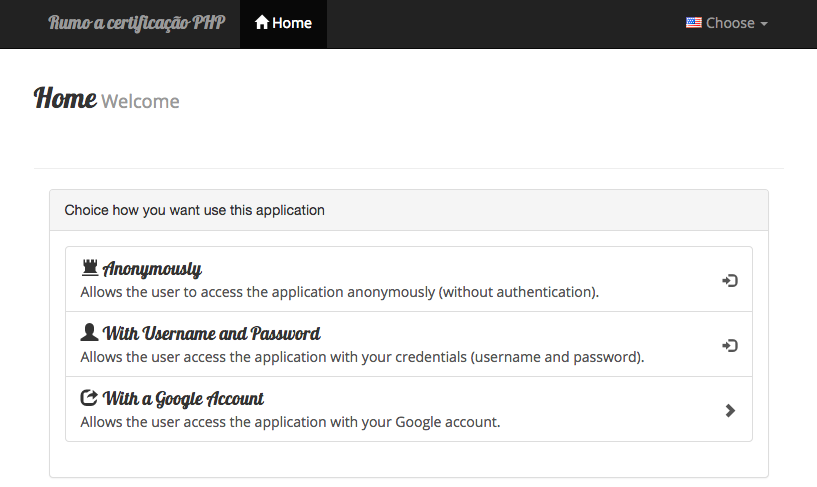
\includegraphics[width=\textwidth]{images/resultados/zcpe-home.png}

	\centering
	\footnotesize Fonte: \fonteOAutor
\end{figure}

\FloatBarrier 	% Este comando impede que as imagens
				% flutuem a partir deste ponto no seu documento

A listagem de perguntas apresentada na Figura \ref{fig:zcpePerguntaListagem} é
o resultado da categorização de perguntas e respostas da lista de discussão,
sendo que, nesta listagem apresentam-se dados básicos para o usuário que está logado, e para os usuários
administradores exibe-se uma coluna adicional ``aprovado'', sendo que, quando
o valor desta coluna é ``Sim'', então a ferramenta libera a questão
para ser utilizada pelo sistema de simulado.

\begin{figure}[h!tb]
	\caption{Listagem de perguntas}
	\label{fig:zcpePerguntaListagem}

	\centering
	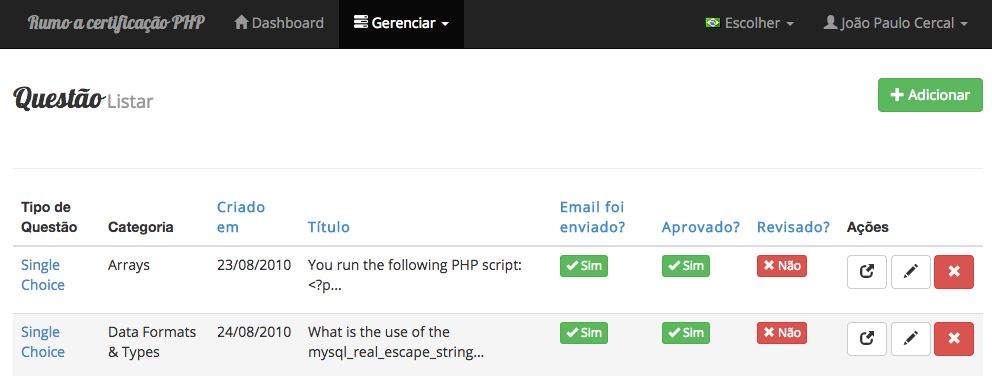
\includegraphics[width=\textwidth]{images/resultados/zcpe-pergunta-listagem.png}

	\centering
	\footnotesize Fonte: \fonteOAutor
\end{figure}

\FloatBarrier 	% Este comando impede que as imagens
				% flutuem a partir deste ponto no seu documento

Na Figura \ref{fig:googleGroupsListagemTopicos}, percebe-se que as questões não
são gerenciadas através de categorias, não há também uma forma de gerenciar as
respostas corretas. Outro problema existente é o fato de que não há somente
perguntas na listagem de tópicos, por conseguinte a ferramenta proposta eliminou estes
problemas.

\begin{figure}[h!tb]
	\caption{Listagem de tópicos no Google Groups}
	\label{fig:googleGroupsListagemTopicos}

	\centering
	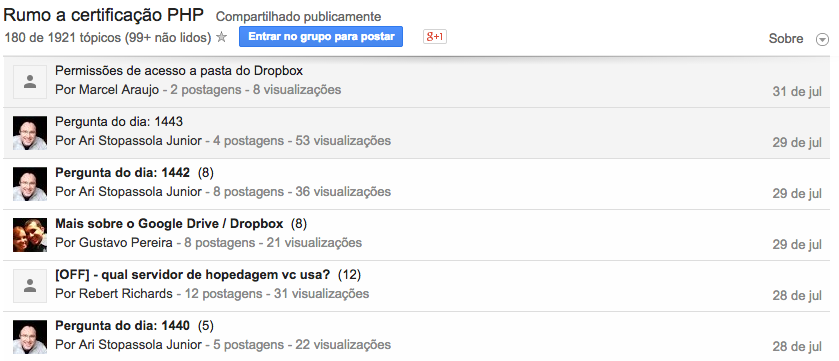
\includegraphics[width=\textwidth]{images/resultados/google-groups-listagem.png}

	\centering
	\footnotesize Fonte: \fonteOAutor
\end{figure}

\FloatBarrier 	% Este comando impede que as imagens
				% flutuem a partir deste ponto no seu documento

Neste momento apresenta-se em detalhes na Figura \ref{fig:zcpePerguntaDetalhes},
a representação da exibição de detalhes de uma questão que está sendo gerenciada
através da ferramenta proposta.

\begin{figure}[h!tb]
	\caption{Detalhes de uma questão}
	\label{fig:zcpePerguntaDetalhes}

	\centering
	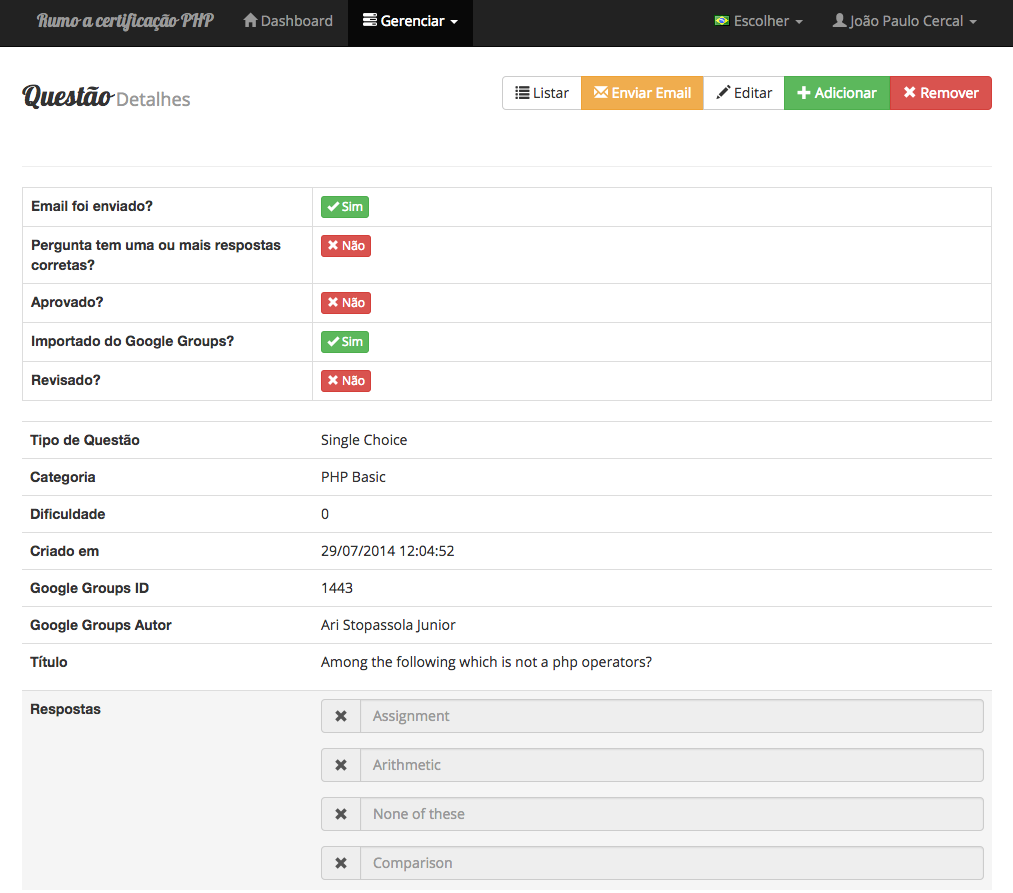
\includegraphics[width=\textwidth]{images/resultados/zcpe-pergunta-detalhes.png}

	\centering
	\footnotesize Fonte: \fonteOAutor
\end{figure}

\FloatBarrier 	% Este comando impede que as imagens
				% flutuem a partir deste ponto no seu documento

Nota-se também que nem todas as informações que o sistema mantém referente a
questão são exibidos na Figura \ref{fig:zcpePerguntaDetalhes}, sendo que, a
linha ``aprovado'' é exibida apenas para os usuários com permissões
administrativas.

A seguir apresenta-se na Figura \ref{fig:zcpePerguntaDetalhesGoogleGroups}, a
mesma questão na plataforma do \textit{Google Groups} no qual não há nenhum gerenciamento das questões que
foram postadas, diferentemente da nova forma de gestão de perguntas proposta por
este projeto.


\begin{figure}[h!tb]
	\caption{Detalhes da questão 1443 no Google Groups}
	\label{fig:zcpePerguntaDetalhesGoogleGroups}

	\centering
	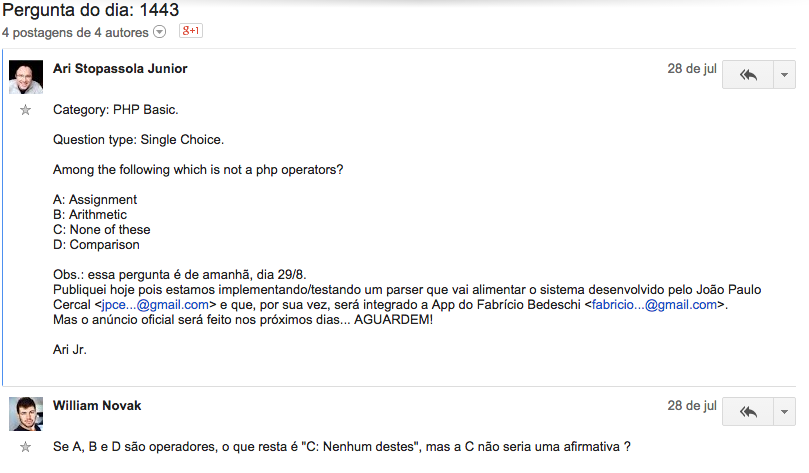
\includegraphics[width=\textwidth]{images/resultados/google-groups-pergunta-1443.png}

	\centering
	\footnotesize Fonte: \fonteOAutor
\end{figure}

\FloatBarrier 	% Este comando impede que as imagens
				% flutuem a partir deste ponto no seu documento
				
Nota-se também que o sistema proposto está internacionalizado e já conta com
dois idiomas, o português do Brasil e o inglês internacional conforme mostra a
Figura \ref{fig:zcpeIdioma}.

\begin{figure}[h!tb]
	\caption{Caixa para seleção do idioma utilizado no sistema}
	\label{fig:zcpeIdioma}

	\centering
	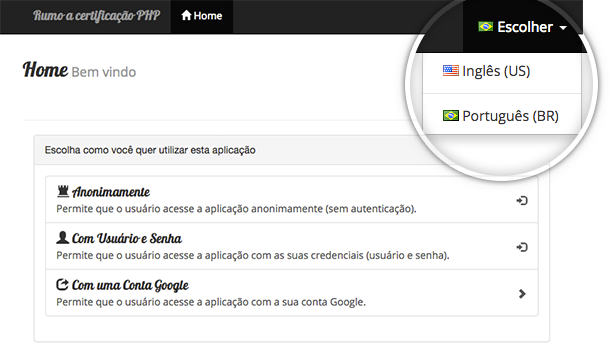
\includegraphics[width=\textwidth]{images/resultados/zcpe-idioma.png}

	\centering
	\footnotesize Fonte: \fonteOAutor
\end{figure}

\FloatBarrier 	% Este comando impede que as imagens
				% flutuem a partir deste ponto no seu documento